\chapter{\uppercase {\aetherflowcap Implementation}}
\label{sec:impl}

\section{Implementation on an AP}


\begin{figure*}[t]
\centering
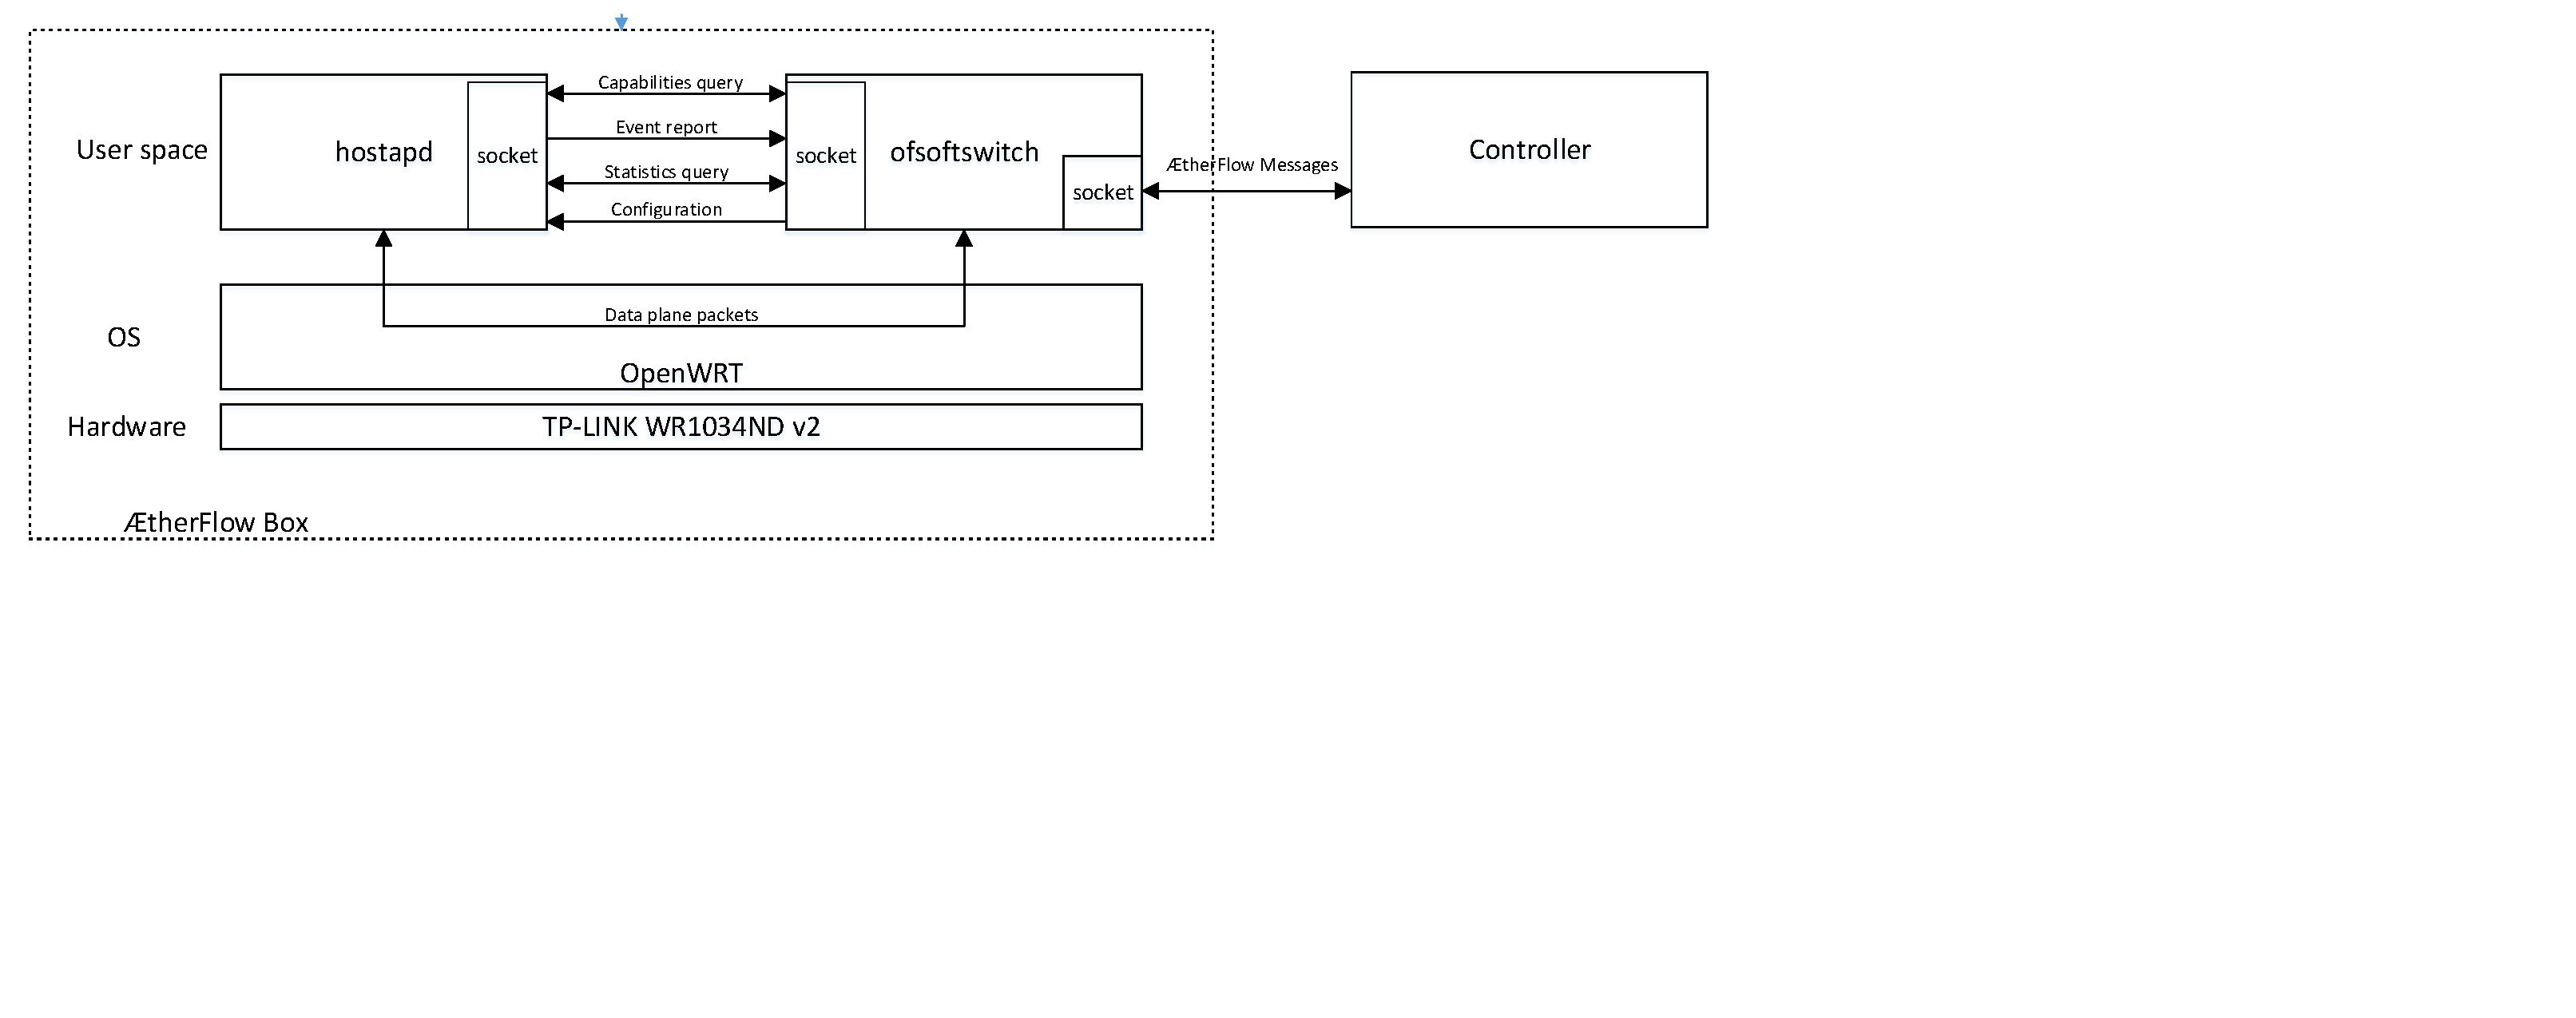
\includegraphics[trim=.2in 3.75in 7in .2in, clip, width=1.0\textwidth]{figures/implementation}
\caption{Implementation of \aetherflow.}
\label{fig:impl}
\end{figure*}

To validate our design and to demonstrate the viability of the \aetherflow
framework as a platform for the development and deployment of intelligent
wireless SDN applications, we implemented and deployed \aetherflow on a commercially
available access point. 

We chose the access point TP-LINK WR1034ND v2 as the hardware 
platform for our implementation.  This AP has five 100Mbps Ethernet ports and one
3-antenna radio interface, supporting protocols IEEE~802.11b/g/n.  We replaced
the firmware of the AP with OpenWRT 14.07 Barrier Breaker. OpenWRT
is an open source Linux distribution designed for network embedded systems.
Network utilities are integrated in OpenWRT and are optimized in size to fit in
embedded environments which usually do not have as much resources as general
purpose computer systems. In OpenWRT, when the radio interface is set up as an
access point, its data plane is managed by Linux kernel and its control plane
is run in the user space by daemon \texttt{hostapd}. 

The native OpenWRT system does not support SDN. To make our access point an SDN
switch, we used the open source CPqD SoftSwitch (\texttt{ofsoftswitch}), which implements an OpenFlow v1.3 pipeline and switch
agent that can be deployed on OpenWRT system.

An \aetherflow data plane extension is then implemented in
\texttt{ofsoftswitch}. The extension adds in wireless physical and logical
ports that are mapped to the radio interface and access points managed by \texttt{hostapd}. To
establish communication between \texttt{ofsoftswitch} and \texttt{hostapd},
\texttt{hostapd} is also modified to enable control of AP from
\texttt{ofsoftswitch} and event reporting from AP to \texttt{ofsoftswitch}. The two
processes communicate via a Unix socket in the OpenWRT system.  An overview of this
implementation is depicted in Figure~\ref{fig:impl}.

Whenever an event related to a mobile station is triggered in \texttt{hostapd},
the event summary is sent to \texttt{ofsoftswitch}, which forwards it to
the controller using the event port message. Whenever a statistics request from the
controller is received by \texttt{ofsoftswitch}, the request is forwarded to
\texttt{hostapd}, and the statistics data is sent to \texttt{ofsoftswitch} and
then sent to the controller with a statistics reply message. Similar behavior
occurs for capability queries and configuration updates.
